% !TeX spellcheck = cs_CZ
%{\tikzset{external/prefix={tikz/FYZI/}}
% \tikzset{external/figure name/.add={ch47_}{}}
%=========================== Kapitola: Zvuk. Vlnová rovnice =======================================
\setchaptertoc
\chapter{Zvuk. Vlnová rovnice}\label{fyz:IchapXLVII}

  \section{Vlny}\label{fyz:IchapXLVIIsecI}
  \section{Šíření zvuku}\label{fyz:IchapXLVIIsecII}
  \section{Vlnová rovnice}\label{fyz:IchapXLVIIsecIII}
  \section{Řešení vlnové rovnice}\label{fyz:IchapXLVIIsecIV}
  \section{Rychlost zvuku}\label{fyz:IchapXLVIIsecV}
  \section{Příklady a cvičení}\label{fyz:IchapXLVIIsecVI}

    \begin{figure}[ht!] %\ref{fyz:fig0457}
      \centering
      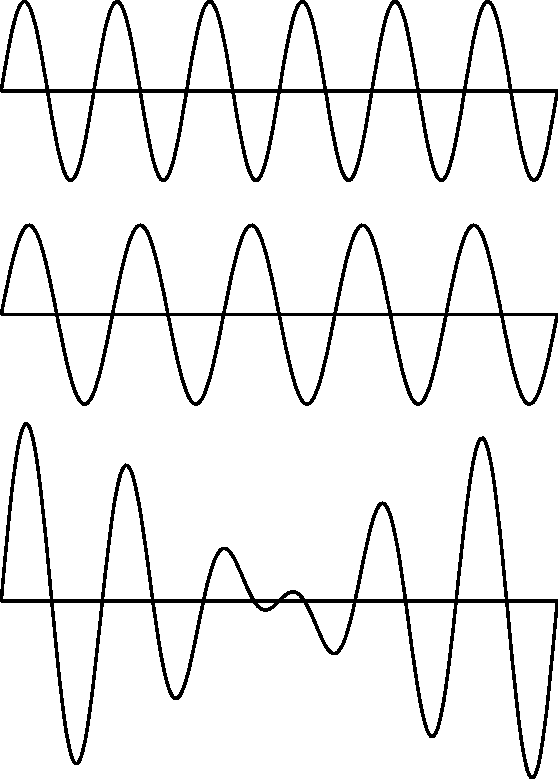
\includegraphics[width=0.7\linewidth]{fyz_fig0457.pdf}
      \caption{ 
               (\cite[s.~707]{Feynman01})}
      \label{fyz:fig0457}
    \end{figure}

    \begin{figure}[ht!] %\ref{fyz:fig0458}
      \centering
      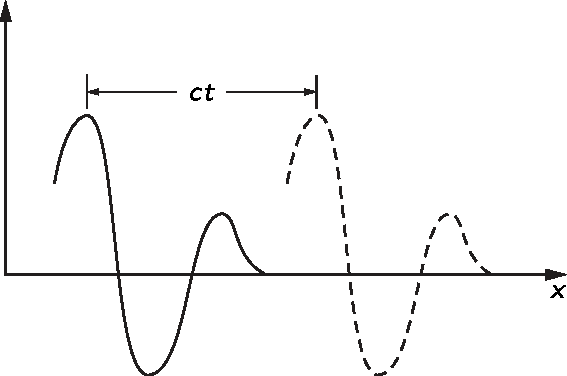
\includegraphics[width=0.7\linewidth]{fyz_fig0458.pdf}
      \caption{ 
               (\cite[s.~707]{Feynman01})}
      \label{fyz:fig0458}
    \end{figure}

    \begin{figure}[ht!] %\ref{fyz:fig0459}
      \centering
      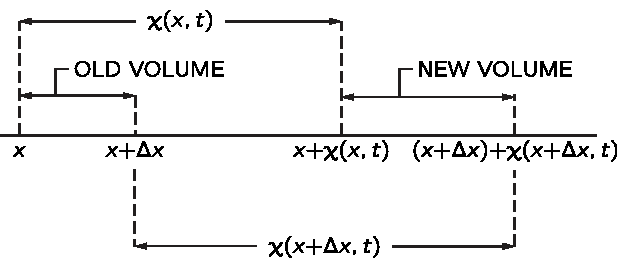
\includegraphics[width=0.7\linewidth]{fyz_fig0459.pdf}
      \caption{ 
               (\cite[s.~707]{Feynman01})}
      \label{fyz:fig0459}
    \end{figure}

    \begin{figure}[ht!] %\ref{fyz:fig0460}
      \centering
      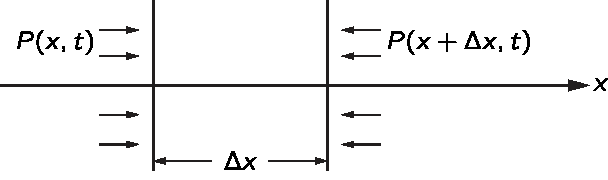
\includegraphics[width=0.7\linewidth]{fyz_fig0460.pdf}
      \caption{ 
               (\cite[s.~707]{Feynman01})}
      \label{fyz:fig0460}
    \end{figure}
    
    \todo[inline]{Kapitola fey1ch47 je zcela prázdná, pouze obrázky} 
%} %tikzset
%---------------------------------------------------------------------------------------------------